%Document Props
%FONT SIZE
%DOC CLASS
\documentclass[12pt, a4paper]{report}

%Packages
\usepackage{fullpage} %1-inch margins
\usepackage{setspace} %double space

% BibLaTeX
%style=ieee looks ugly
\usepackage[backend=bibtex8]{biblatex}
\addbibresource{ref.bib}

%Change Chapter format in report class
\usepackage{titlesec} 
\titleformat{\chapter}[block]
  {\normalfont\huge\bfseries}{\thechapter.}{1em}{\Huge}
\titlespacing*{\chapter}{0pt}{-19pt}{0pt}

%Graphics package and relative path
\usepackage{graphicx}
\graphicspath{{images/}}

% For other font sizes
% !incompatible with fullpage
%\usepackage{extsizes}

% comments
\usepackage{verbatim}

% Hyperlinks package
\usepackage[hidelinks]{hyperref}

\onehalfspacing
% ----------------------------------------------------------------------------------------------
\begin{document}

% Outer Cover Page
\pagestyle{empty}
\begin{titlepage}
\vspace*{0.2cm}
\begin{center} \textbf{A REPORT\\ON} \end{center}
\begin{center} \textbf{{\Large AUTOMATIC LAND COVER CLASSIFICATION OF TEMPORAL SATELLITE IMAGES}} \end{center}
\begin{center} \textbf{BY} \end{center}
\begin{center} 
{\Large 
	\begin{tabular}{c c}
	Guntaas Singh & 2018A7PS0269P\\
	Nisarg Vora & 2018A7PS0254P
	\end{tabular}
}
\end{center}
\begin{center} \textbf{AT} \end{center}
\begin{center} 
\includegraphics{iirs.png} \end{center}
\begin{center} {\Large Indian Institute of Remote Sensing, Dehradun} \end{center}
\begin{center} A Practice School - I station of \end{center}
\begin{center} {
\includegraphics{bits.png}} \end{center}
\begin{center} {\Large Birla Institute of Technology and Science, Pilani} \end{center}
\begin{center} June, 2020 \end{center}
\end{titlepage}
\pagebreak

% Inner Cover Page
\begin{titlepage}
\vspace*{0.3cm}
\begin{center} \textbf{A REPORT\\ON} \end{center}
\begin{center} \textbf{{\Large AUTOMATIC LAND COVER CLASSIFICATION OF TEMPORAL SATELLITE IMAGES}} \end{center}
\begin{center} \textbf{BY} \end{center}
\begin{center}
	\begin{tabular}{c c c}
		\textbf{ID Number} & \textbf{Name} & \textbf{Branch} \\
		2018A7PS0269P & Guntaas Singh & B.E. (Hons.) Computer Science \\
		2018A7PS0254P & Nisarg Vora  & B.E. (Hons.) Computer Science \\
	\end{tabular} 
\end{center}
\begin{onehalfspace}
\begin{center} \textbf{Prepared in the partial fulfillment of the} \end{center}
\begin{center} Practice School - I course \end{center}
\begin{center} \textbf{AT} \end{center}
\begin{center} 
\includegraphics{iirs.png} \end{center}
\begin{center} {\Large Indian Institute of Remote Sensing, Dehradun} \end{center}
\begin{center} A Practice School - I station of \end{center}
\begin{center} {
\includegraphics{bits.png}} \end{center}
\begin{center} {\Large Birla Institute of Technology and Science, Pilani} \end{center}
\begin{center} June, 2020 \end{center}
\end{onehalfspace}
\end{titlepage}
\pagebreak

% Acknowledgements
\setcounter{secnumdepth}{0}
\section{Acknowledgments}
\pagestyle{plain}
\pagenumbering{roman}
\setcounter{page}{3}
We would sincerely like to thank the Director of Indian Institute of Remote Sensing, Dr. Prakash Chauhan, for giving us an opportunity to work in this organization and gain exposure to corporate work culture, ethics, and etiquette to be followed while working in a professional environment.
\paragraph{}
We would like to extend our most sincere gratitude to our project in-charge, Dr. Hari Shanker Srivastava, Head of the Programme Planning and Evaluation Group (PPEG) at IIRS, for providing us with the opportunity to work with him on this project, and his guidance and mentorship during the same.
\paragraph{}
We wish to extend our gratitude to the faculty in charge of the PS-I program at IIRS, Rekha A., Assistant Professor at BITS Pilani - Bangalore Center, for her guidance and advice during the PS-I program, and her helpfulness and responsiveness while addressing all the concerns we raised during the same.
\paragraph{}
In addition, we would also like to thank the members of the Practice School Division, who worked very hard for operating the PS-I programme remotely to ensure that we have a seamless learning experience.
\begin{flushright}
Guntaas Singh\\
Nisarg Vora
\end{flushright}
\pagebreak

% Details and abstract
\begin{center}  
\textbf {BIRLA INSTITUTE OF SCIENCE AND TECHNOLOGY\\
PILANI (RAJASTHAN)\\
Practice School Division}
\end{center}
\begin{onehalfspace}
\textbf{Station:} Indian Institute of Remote Sensing \\
\textbf{Centre:} Dehradun\\
\textbf{Duration:} 3 weeks\\
\textbf{Date of start:} 18th May, 2020 \\
\textbf{Date of submission:} 5th June, 2020 \\
\textbf{Title of project:} Automatic Land Cover Classification of Temporal Satellite Images
\begin{center}
\begin{tabular}{c c c}
\textbf{ID Number} & \textbf{Name} & \textbf{Branch} \\
2018A7PS0269P & Guntaas Singh & B.E. (Hons.) Computer Science \\
2018A7PS0254P & Nisarg Vora  & B.E. (Hons.) Computer Science \\
\end{tabular} 
\end{center}
\textbf{Name of guide:} Dr. Hari Shanker Srivastava \\
\textbf{Designation:} Scientist/Engineer - SG. Group Head, Programme Planning and Evaluation Group (PPEG). \\
\textbf{Name of PS faculty:} Rekha A. \\
\textbf{Key Words:} Semantic Segmentation, Support Vector Machines, Convolutional Neural Networks, U-Net Architecture\\
\textbf{Project Areas:} Remote Sensing, Machine Learning, Deep Learning
\section{Abstract}
\paragraph{}
This project attempts automatic land cover classification of different parts of India into urban, agricultural, forest, water bodies etc which can be used for various applications like natural resource management, urban expansion etc.  Data from Agra district, Uttar Pradesh has been used to train Support Vector Machines and Convolutional Neural Networks which are then tested on Gandhinagar district, Gujarat. Google Earth Engine has been used to obtain data from Landsat 8 satellite images. For the purpose of classification Normalized Difference Vegetation Index (NDVI) values are calculated by masking all other light bands except near-infrared and red light bands. Temporal images with NDVI labellings are fed as an input to the models and the subsequent accuracy of the models is then reported.
\end{onehalfspace}
\newpage

%Response sheet
\begin{comment}
	\begin{center}  
	\textbf {BIRLA INSTITUTE OF SCIENCE AND TECHNOLOGY\\
	PILANI (RAJASTHAN)\\
	Practice School Division\\
	Response Option Sheet}
	\end{center}
	\begin{onehalfspace}
	\textbf{Station:} Indian Institute of Remote Sensing \\
	\textbf{Centre:} Dehradun
	\begin{center}
	\begin{tabular}{c c c}
	\textbf{ID Number} & \textbf{Name} & \textbf{Branch} \\
	2018A7PS0269P & Guntaas Singh & B.E. (Hons.) Computer Science \\
	2018A7PS0254P & Nisarg Vora  & B.E. (Hons.) Computer Science \\
	\end{tabular} 
	\end{center}
	\textbf{Title of project:} Automatic Land Cover Classification of Temporal Satellite Images\\''
	\vspace*{1cm}
	Usefulness of the project to the on-campus courses of study in various disciplines. Project should be scrutinized keeping in view the following response options. Write Course No. and Course Name against the option under which the project comes.\\
	\begin{center}
	\begin{tabular}{|p{1cm}|p{10cm}|p{3cm}|}
	\hline
	\textbf{Code No.} & \textbf{Response Option} & \textbf{Course No.(s) and Name} \\
	\hline
	1 & A new course can be designed out of this project. & ~\\
	\hline
	2 & The project can help modification of the course content of some of the existing Courses & ~\\
	\hline
	3 & The project can be used directly in some of the existing Compulsory Discipline Courses (CDC)/ Discipline Courses Other than Compulsory (DCOC)/ Emerging Area (EA), etc. Courses & ~\\
	\hline
	4 & The project can be used in preparatory courses like Analysis and Application Oriented Courses (AAOC)/ Engineering Science (ES)/ Technical Art (TA) and Core Courses. & ~\\
	\hline
	5 & This project cannot come under any of the above mentioned options as it relates to the professional work of the host organization. &~ \\
	\hline
	\end{tabular} 
	\end{center}
	\end{onehalfspace}
	\vspace*{0.5cm}
	\textbf{Signature}\\
	\textbf{Date: }
	\newpage
\end{comment}

% Table of Contents
\tableofcontents
\listoffigures

% INTRODUCTION
\setcounter{page}{1}
\setcounter{secnumdepth}{2}
\chapter{Introduction}
\pagenumbering{arabic}
\section{About IIRS}
Formerly known as Indian Photo-interpretation Institute (IPI), the Institute was founded on 21st April 1966 under the aegis of Survey of India (SOI). It was established with the collaboration of the Government of The Netherlands on the pattern of Faculty of Geo-Information Science and Earth Observation (ITC) of the University of Twente, The Netherlands. The original idea of setting the Institute came from India's first Prime Minister Pandit Jawahar Lal Nehru during his visit to The Netherlands in 1957. 
\paragraph{}
Since its establishment in 1966, IIRS is a key player for training and capacity building in geospatial technology and its applications through training, education and research in Southeast Asia. The training, education and capacity building programmes of the Institute are designed to meet the requirements of professionals at working levels, fresh graduates, researchers, academia, and decision makers.
\cite{iirs.about.history, iirs.about.instiprof}
\section{Remote Sensing}
Remote sensing is the method of getting information about Earth and its surface without making any physical contact, primarily using satellites. Remote sensing is used in numerous fields, including geography, land surveying and most Earth science disciplines (for example, hydrology, ecology, meteorology, oceanography, glaciology, geology); it also has military, intelligence, commercial, economic, planning, and humanitarian applications.\cite{remotesensingwiki}
It may be split into "active" remote sensing and "passive" remote sensing. In active remote sensing method, sensors are used to capture the reflection of the signals emitted by the satellite on different objects. In passive remote sensing, the reflection captured by the sensors is mainly due to sunlight. In this project, we are using passive remote sensing by Landsat 8 satellite.

\section{Objective: Land Cover Classification}
Land Cover classification generally refers to the categorization or classification of human activities and natural elements on the landscape within a specific time frame based on established scientific and statistical methods of analysis of appropriate source materials.Land cover refers to the surface cover on the ground like vegetation, urban infrastructure, water, bare soil etc. identification of land cover establishes the baseline information for activities like thematic mapping and change detection analysis.\cite{landcoversig}
\subsection{Techniques}
Mainly two techniques are used for land cover classification: Field survey and Remotely sensed imagery analysis. Field survey was the primary method used for land cover classification until a few decades back however it was very inaccurate and time-consuming.With developments in technology, conventional method of field survey which is both inaccurate and time consuming has been replaced by remotely sensed imagery analysis which is highly accurate and covers wider range.

\begin{figure}[h]
\centering
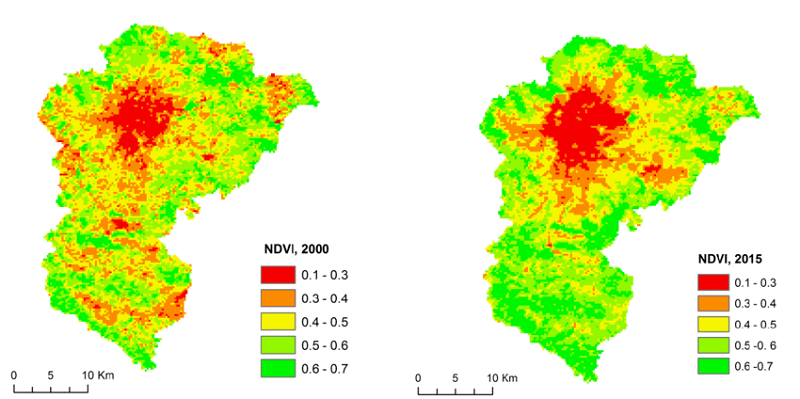
\includegraphics[width=\textwidth]{landcover.png}
\caption{NDVI distribution in 2000 and 2015 in Kathmandu valley, Nepal, derived from MODIS data.}
\cite{lcimg}
\end{figure}
\subsection{Significance}
Land cover classification data is of great importance in the following applications:
\begin{itemize}
\item \textbf{Natural Resource Management:} Land cover classification can help policy makers decide how to best manage all the available resources by looking at different terrains. For example government can decide which area requires irrigation facilities the most using land cover classification. 
\item \textbf{Wildlife habitat protection:} With shrinking habitats of wild animals land cover classification can provide important data for helping in wildlife preservation and protection.
 \item \textbf{Urban Expansion/encroachment:} Proper planning is required for expansion of urban area and different land cover features need to be studied to minimize the time and economic cost required for tackling natural obstacles to urban expansion.
 \item \textbf{Damage delineation (Tornadoes, flooding, fire, volcanic):} Live land cover data can provide us information about where a certain natural disaster like flood has occurred/can occur and where has it cause damages.
 \item \textbf{Target Detection - identification of land strips for use:} Using land cover data, identification of ideal locations for different urban construction becomes easy. For example one can decide where exactly it is possible to build an airport or bridge etc.
\end{itemize}

\newpage

% ____________________________

% METHODOLOGY
\chapter{Methodology}

\section{Normalized Difference Vegetation Index(NDVI)}
Satellite data has become a  very important parameter for judging crop progress, land cover classification etc. However, satellite data can not directly report crop health or classify land cover into different classes. NDVI which is calculated by measuring the reflectance of near-infrared and red light is probably the most important and accurate parameter for farmers to know crop health. NDVI values are so accurate that they can in fact, inform farmers about upcoming drought 2 weeks in advance. Farmers can then make corresponding decisions to increase irrigation and other crop supplements.
\paragraph{}
NDVI values can provide really useful and accurate information about crop health to the concerned authorities and can also help in making predictions of upcoming drought. Evapotranspiration (ET) is another satellite data that can used however, it suffers from one drawback as compared to NDVI values. NDVI values are available on a monthly basis whereas evapotranspiration values are only available monthly, making NDVI measurements more accurate. 
\subsection{What is NDVI?}
Light from the sun falls on Earth in three major light bands: Ultraviolet, infrared and red. Most of the ultraviolet is reflected back by the atmosphere. Healthy green plants absorb most of the visible light for photosynthesis however, to prevent over-heating and dehydration the light in red band and near-infrared band is reflected back by the plants. The red light is visible to human and not the infrared. The NDVI values are calculated using the reflectance in red and near-infrared regions.
\subsection{Formula}
NDVI is calculated in accordance with the formula:
\begin{displaymath}
NDVI=\frac{NIR-RED}{NIR+RED}
\end{displaymath}
where,\\
$NIR=$ reflection in the near-infrared spectrum\\
$RED=$ reflection in the red range of the spectrum.
\paragraph{}
As per the formula above, the density of vegetation (NDVI) at a certain point of the image is equal to the difference in the intensities of reflected light in the red and infrared range divided by the sum of these intensities.\\
NDVI values range from -1.0 to 1.0, the positive values are usually for plants and vegetation where as the negative values usually indicate presence of snow, water or cloud cover. Values very close to 0 and less than 0.1 are due to presence of urban built ups rocks etc. Moderate values between 0.2 and 0.3 are due to shrubs and crops whereas large values close to 1.0 represent temperate and tropical forests. 
\begin{figure}[ht!]
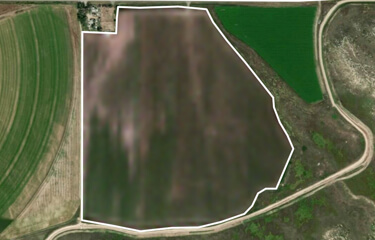
\includegraphics[width=.45\textwidth]{ndvisampleone.jpg}\hfill
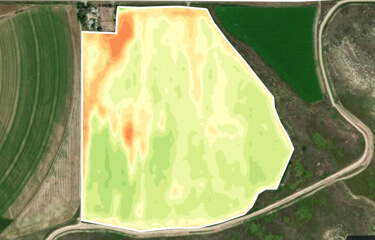
\includegraphics[width=.45\textwidth]{ndvisampletwo.jpg}
\caption{(1) Without NDVI. (2) With NDVI.}
\end{figure}
\begin{figure}[h]
\centering
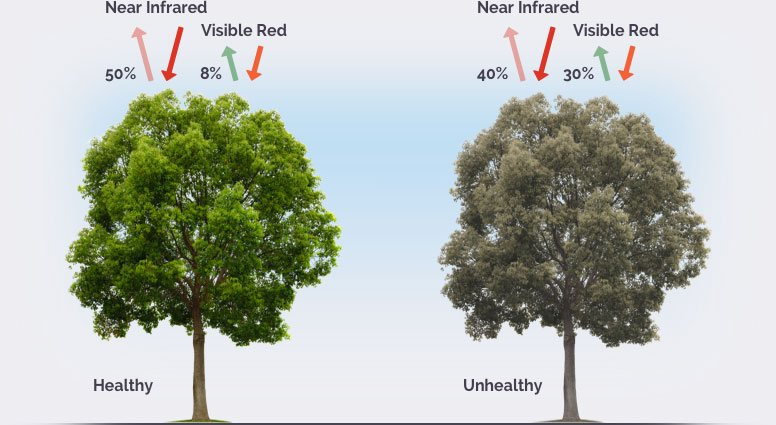
\includegraphics[width=0.8\textwidth]{ndviillustration.jpg}
\caption{Plant health directly affects reflectance in NIR and RED bands.}
\end{figure}
\subsection{Correlation with plant health}
The amount of chlorophyll acts as an health indicator for the plants. Chlorophyll strongly absorbs visible light and the cell structure reflects near-infrared light. When chlorophyll levels are low, the cell structure gets destroyed and starts absorbing near-infrared light instead of reflecting it. Thus, value of NIR without vegetation decreases and hence the NDVI value becomes smaller.

\section{Image Classification}
Image classification is a standard task in computer vision. In general, the image classification problem involves assigning one  label out of a given fixed set of discrete labels to the input image on the basis of its visual content. While this is a trivial task for humans, robust image classification is a big challenge for a machine. To the computer, the image is just a grid of numbers which entirely change in unreliable ways with variations in viewpoint, illumination, occlusion, etc. As a result, there is no obvious algorithm which solves this problem. However, a data driven approach of providing the machine with many examples of each class and use of machine learning techniques has shown to be useful.\cite{cs231n}
\paragraph{}
There are different ways in which these techniques can be applied for classification of satellite imagery.
\subsection{Pixel Based Approach}
In typical satellite images, pixel sizes are generally similar in size to the objects of interest. Most of the methods for image analysis using remote sensing data work on a per-pixel basis. However, with advances in remote sensing technology, the spatial resolution has become finer than the typical objects of interest, leading to an increase in within-class variability.\cite{eyesky}
\subsection{Object Based Approach}
The term "objects" represents meaningful semantic entities or scene components that are distinguishable in an image.\cite{eyesky} This approach involves the partition of the image into meaningful geographical objects that share relatively homogeneous spectral, color, etc.
\subsection{Semantic Approach}
This aims to label each scene image with a specific semantic class. Here, a scene image usually refers to a local image patch manually extracted from large scale remote sensing images that contain explicit semantic classes.\cite{eyesky}

\section{Supervised Machine Learning}
Supervised learning is the machine learning task of learning a function that maps an input to an output based on example input-output pairs.\cite{supervisedlearningone} Supervised learning is the machine learning task of learning a function that maps an input to an output based on example input-output pairs.\cite{supervisedlearningtwo} If enough data is available then the trained model usually identifies the underlying data patterns and is then able to make predictions on previously unknown input. The training data is the set of input-output example pairs used to train the classifier. Supervised learning, however, faces the problem of overfitting when model is made very flexible in order to fit the underlying data and underfitting when the model is to rigid to fit the underlying data.
\section{Support Vector Machines}
A Support Vector Machine (SVM) is a discriminative classifier formally defined by a separating hyperplane. In other words, given labeled training data (supervised learning), the algorithm outputs an optimal hyperplane which categorizes new examples. In two dimentional space this hyperplane is a line dividing a plane in two parts where in each class lay in either side.\cite{supportvectormachines}
\subsection{Types of SVMs}
There are two kinds of support vector machines: Hard Margin Support Vector Machines and Soft Margin Support Vector Machines.
Hard Margin Support Vector machines do not allow misclassification of data points, tend to overfit the data and are thus sensitive to outliers. Soft margin support vector machines allow slight misclassification of data points and penalize for each misclassification.
For this project, soft margin support vector machines have been used to classify the data points.
\begin{figure}[h]
\centering
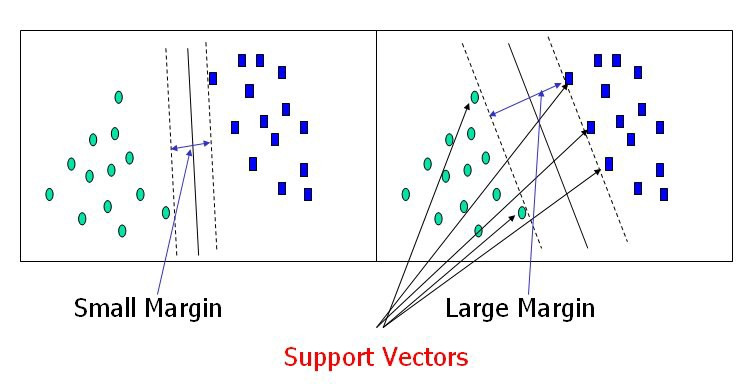
\includegraphics[width=0.7\textwidth]{supportvectormachines.jpg}
\caption{Support Vector Machine}
\end{figure}
\subsection{Advantages}
The advantages of using support vector machines are:
\begin{itemize}
\item Support vectors can deal with high dimensional data easily with the help of kernel transformations.
\item They are only dependent on some part of the training data known as the support vectors which makes them very memory efficient.
\item Can be used for a variety of tasks due to availability of a large number of kernel functions for decision making.
\item Fast and memory efficient implementations in various languages is available via different libraries.
\end{itemize}
\subsection{Disadvantages}
The disadvantages of using support vector machines are:
\begin{itemize}
\item They do not take the spatial orientation of the pixels into account while learning.
\item With wrong choice of kernel, support vector machines tend to to overfit the data.
\item Hard margin support vector machines are very sensitive to outliers and hence proper care should be taken while using them.
\end{itemize}

\newpage
\section{Deep Learning and Neural Networks}
Application of traditional machine learning techniques requires handcrafted features, developing which demands a considerable amount of engineering skill and domain expertise. This, however, is not true for neural networks, which automatically learn these features from data using a general-purpose learning procedure.\cite{eyesky, cs231n} 
%Despite having been around for decades, neural networks have garnered much attention only in the last few years on account of the availability of increased computational power and large amounts of data.
\paragraph{}
A standard neural network consists of many simple, connected processors called neurons, each producing a sequence of real-valued activations. Input neurons get activated through data applied at the input of he network. Other neurons get activated through weighted connections from previously active neurons. \cite{schmidhuber2015deep} Each neuron can be seen as a single unit applying a non-linear activation function (such as sigmoid, tanh, ReLU) to a linear combination of the input activations to the neuron.\cite{cs229}
\begin{figure}[h]
\centering
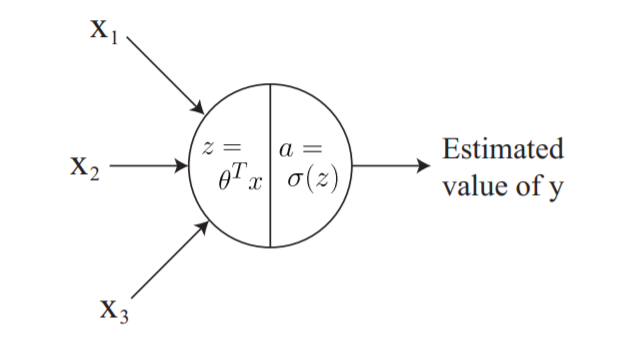
\includegraphics[width=0.5\textwidth]{nn1.png}
\caption{A single neuron.}\cite{cs229}
\end{figure}
\paragraph{}
These single neurons can be stacked so that one neuron passes its output as input into the next neuron. The resulting network of neurons can, hence, consist of several layers of neurons, each with their own learnable weights and biases. Used in conjunction with an appropriate loss function and optimization algorithm, such a network can be used to learn any complex function, if sufficient data is available for training. Forward propagation through the network yields its prediction for a given input. This prediction is compared with the actual class label, and the loss is computed. Backward Propagation is used to compute the gradients of the loss function with respect to the parameters, which are then used by the optimization algorithm to adjust the parameters and minimize the loss over a number of iterations.
\begin{figure}[h]
\centering
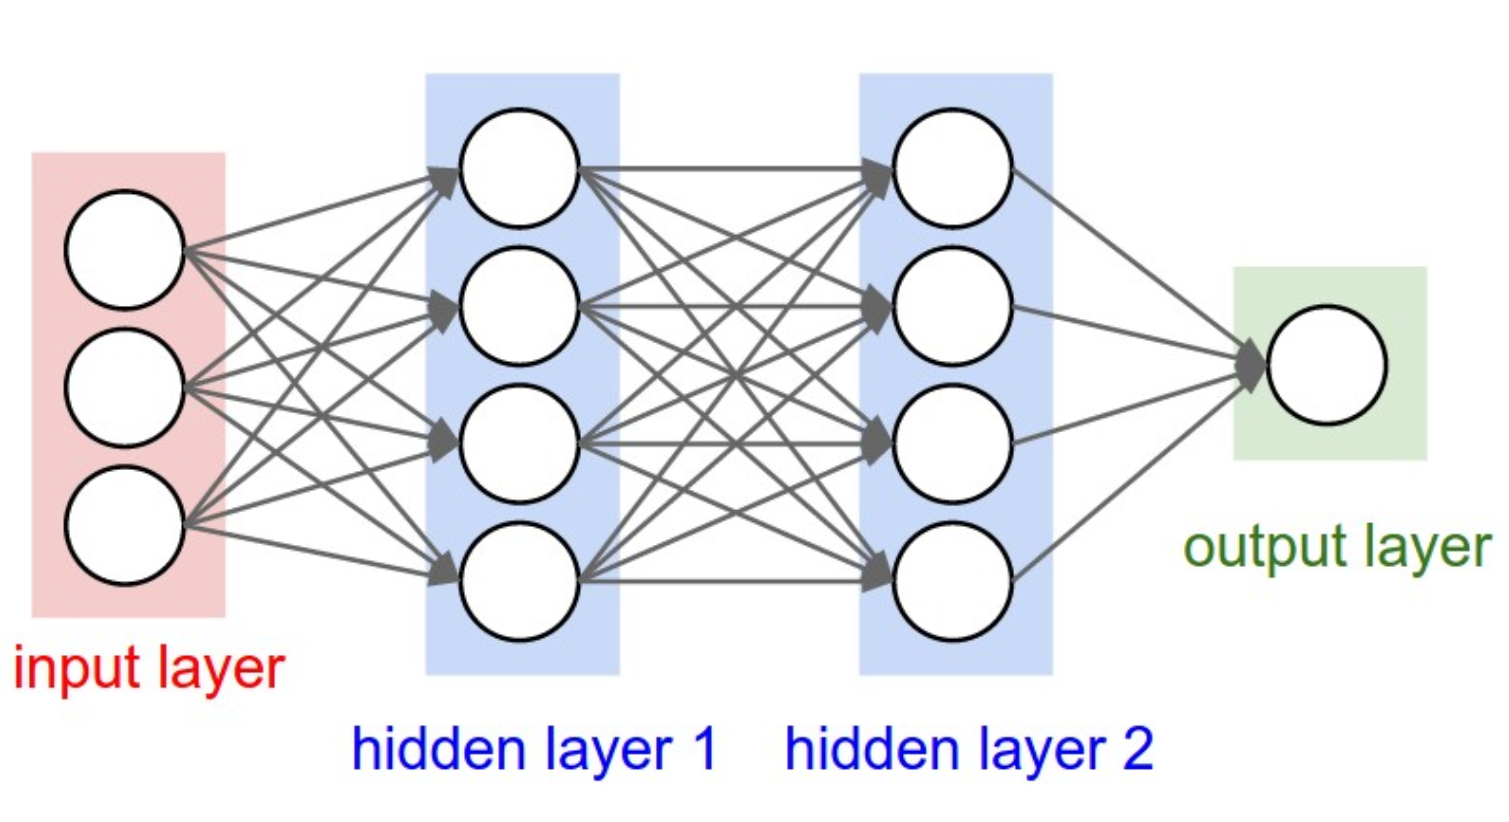
\includegraphics[width=0.7\textwidth]{nn2.png}
\caption{A two layer neural network with fully connected layers.}\cite{cs231n}
\end{figure}
\newpage

\section{Convolutional Neural Networks}
Regular neural networks do not scale well to full images. If the input to the neural network is a 200x200 RGB image, the number of weights for each neuron will be 200*200*3 = 120,000 weights. For large networks, the total number of learnable parameters become very large and lead the model to potentially overfit the training data, unless the training set is adequately large.
\paragraph{}
A convolutional neural network (CNN) is a sequence of layers. Each layers transforms an input volume (images are represented as a three dimensional matrix) of activations to another with some differentiable function which may or may not have parameters.\cite{cs231n, dlai4} These layers are of three main types:
\subsection{Convolutional Layer}
This is the core building block for convolutional networks. It is based on the convolution operation on images.
\paragraph{}
Each convolutional layer of a CNN consists of $N$ kernels or filters of a certain volume of neurons sized $f \times f \times d$, with $f$ being the spatial dimension and $d$ being the number of feature channels of the kernel, which is same as the number of channels in the image at its input ($D_{i}$). Every one of these filters is slid through the entire image of size $H_{i} \times W_{i} \times D_{i}$. Convolution refers to the summation of the element-wise dot product of the neurons in each filter with the corresponding values in the input, for each position in which the filter is aligned with the image. Based on this notion, a convolution with a single filter at each layer results in a two dimensional output of a certain size. \cite{cs231n, muruganandham2016semantic, dlai4}
\begin{figure}[h]
\centering
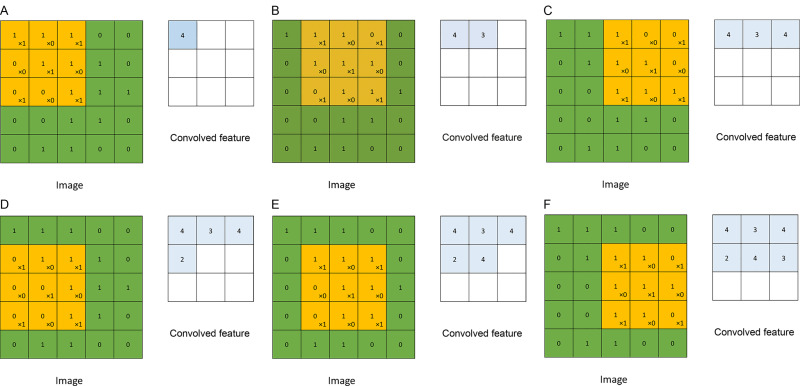
\includegraphics[width=\textwidth]{cnn1.jpg}
\caption{The convolution operation performed using a 3x3 filter on a 5x5x1 image.}\cite{fathi2018deep}
\end{figure}
\paragraph{}
The intervals with which the filter moves in each spatial dimension is decided by the \textbf{stride} $s$. In order to prevent undue shrinkage of the volume along the spatial dimension, the image can be padded with pixels along the outer edges. The width of this \textbf{padding}, in pixels, is given by another hyper-parameter, $p$.\cite{dlai4, muruganandham2016semantic} The convolution operation is repeated for each of the $N$ filters, and the resulting $N$ activation maps are stacked together across the third dimension giving an output volume of dimensions:\\
\begin{displaymath}
H_{o}=\frac{H_{i}-f+2p}{s}+1
\end{displaymath}
\begin{displaymath}
W_{o}=\frac{W_{i}-f+2p}{s}+1
\end{displaymath}
\begin{displaymath}
D_{o}=N
\end{displaymath}
\paragraph{}
In a convolutional layer, each neuron is connected to only a local region of the input volume, called the receptive field of that neuron. The extent of connectivity is limited to the filter size along the spatial dimensions, but is full along the depth axis.\cite{cs231n} It should also be noted that all activations belonging to a particular channel in the output volume correspond to a single filter applied on the input volume, and hence depend on the same shared parameters. Local connectivity and parameter sharing not only help reduce the number of learnable parameters, but also make the CNN good at capturing \textbf{translation invariance}. This makes them an ideal choice for the image classification problem.
\subsection{Pooling Layer}
It is common to periodically insert a Pooling layer in-between successive convolutional layers in a CNN. Its function is to progressively reduce the spatial size of the representation to reduce the amount of parameters and computation in the network, and hence to also control overfitting.\cite{cs231n} The most common form of pooling layer in CNN architectures employs filters of size $2 \times 2$ with a stride of 2, taking a max over 4 cells of the input image. It is worth noting that while this halves the width and height of the image, the depth remains unaffected as the max operation is applied independently to each channel of the image. This down-sampling process effectively discards 75\% of the activations.
\begin{figure}[h]
\centering
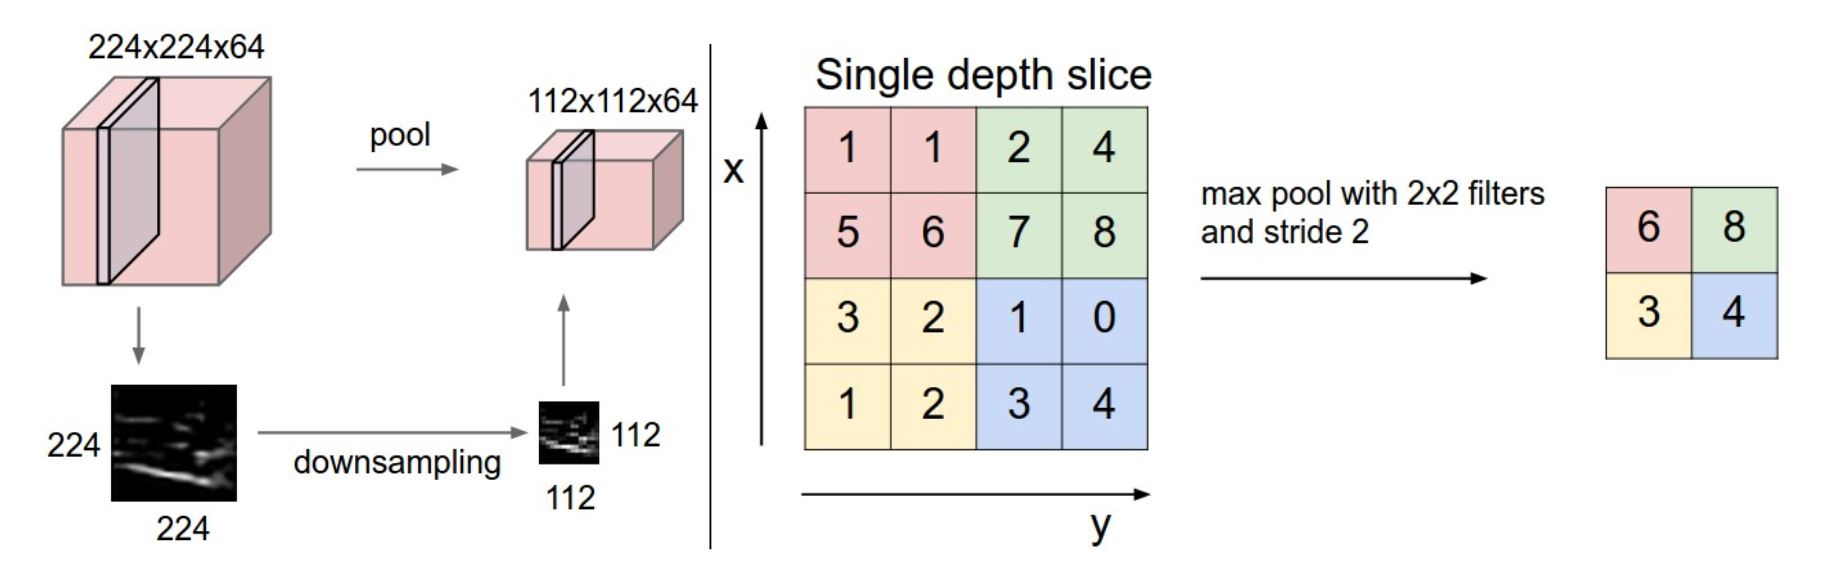
\includegraphics[width=\textwidth]{cnn2.jpg}
\caption{(1) A typical max pooling layer. (2) The max pooling operation.}\cite{cs231n}
\end{figure}
\subsection{Fully Connected Layer}
Once higher level features are detected from the preceding convolution and pooling layers, a fully connected layer is usually attached at the end of the network. This layer is fully connected to all activations in the previous layer, as in regular neural networks, allowing all the features learned by the network to be taken into account by the output layer.
\paragraph{}
All of these different types of layers can be stacked together in various ways to form a CNN.
\begin{figure}[h]
\centering
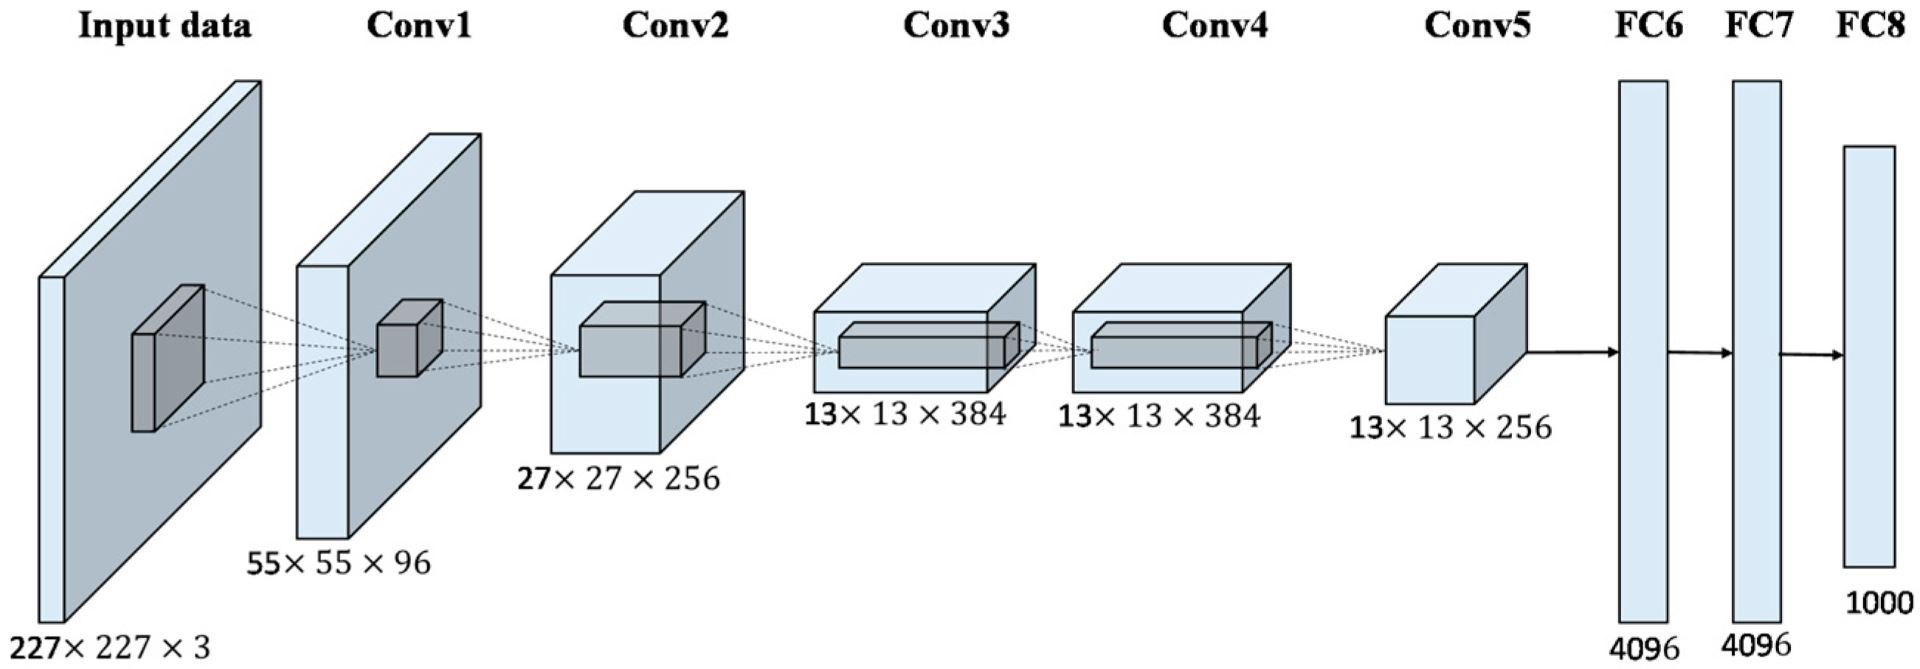
\includegraphics[width=\textwidth]{cnn3.jpg}
\caption{AlexNet - an influential NN architecture that popularized the use of CNNs and GPUs to accelerate deep learning.}\cite{alexnet, alexnetimg}
\end{figure}

\section{Semantic Segmentation}
Typical CNNs used for image classification take fixed-size inputs and produce non-spatial outputs (predicted class labels). However, in case of land cover classification, the objective is not to assign a single class label to a given satellite image, but to divide the given image into segments each corresponding to one class out of a given set of land cover classes. This problem is known as semantic segmentation. There are different ways in which the existing image classification CNNs can be extended to solve this problem.
\paragraph{}
One approach is to use networks with only convolutional layers. In these networks, zero padding can be used to preserve the spatial dimensions of the input image. However, the large spatial dimensions throughout the network make the model computationally infeasible. \cite{long2015fully, cs231n, unet}
\paragraph{}
While the problem requires the CNN to produce a spatial output, down-sampling is essential for reducing the need for computational resources to a feasible level. As a result, the most popular approach is to design the network as a combination of an encoder(down-sampling path) and a decoder(up-sampling path).\\

\section{FCN Architecture}
Fully connected layers have an equivalent representation as a convolutional layer having $N$ filters with dimensions equal to those of the input image. The output of this layer will thus be a volume of dimensions $1 \times 1 \times N$. This simple change allows the same CNN to be applied on images with arbitrary spatial dimensions and classify them in a single pass of forward propagation. This is far more efficient than iterating on different crops and classifying one pixel at a time. This is the basic intuition behind \textbf{Fully Convolutional Networks}.\cite{long2015fully} For up-sampling the classification maps produced by a FCN, \textit{Long et al.}\cite{long2015fully} propose the use of transpose convolution. 
\subsection{Transpose Convolution}
Ordinary convolution involves taking a dot product between the filter and the input for every receptive field at a stride of s in the input, and storing the result at a stride of 1 in the output. The resulting output image gets down-sampled by a factor of s. In transpose convolution, we use the values at a stride of 1 in the input and take their scalar product with the filter, storing the resulting matrix at a stride of s in the output. As a result the image gets up-sampled by a factor of s. Any overlapping values in the output are summed together.\cite{long2015fully, cs231n}
A stack of layers performing transpose convolution with an appropriate activation function can be used to learn a non-linear up-sampling.\cite{long2015fully}\begin{figure}[h]
\centering
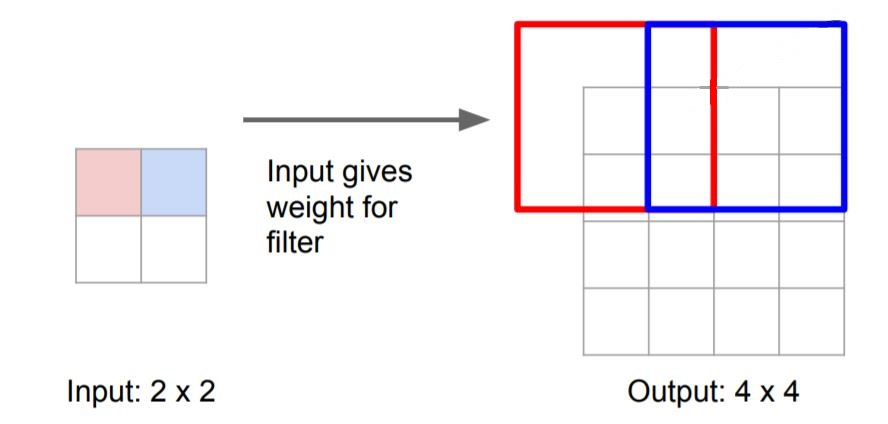
\includegraphics[width=0.7\textwidth]{fcn.jpg}
\caption{A $3 \times 3$ transpose convolution with stride 2 and padding 1. The output gets up-sampled by a factor of 2.}
\cite{cs231n}
\end{figure}
\subsection{Skip Connections}
Semantic segmentation faces an inherent tension between semantics and location. Deep layers capture local information and resolve the semantic information that the image contains. Global information available to shallower layers can be used to capture the location. This motivates the idea of adding skip connections from shallow layers to the final prediction layer. Combining the information captured by shallow and deep layers at the time of up-sampling lets the model make local predictions that take into account global structure and semantics. To combine activations with different spatial dimensions, they are first up-sampled individually as required using transpose convolutions and then summed up. The result is then up-sampled by a final layer, so that the output spatial dimensions match those of the input image. The addition of skip connections produces a finer and more detailed segmentation map.\cite{long2015fully}
\begin{figure}[h]
\centering
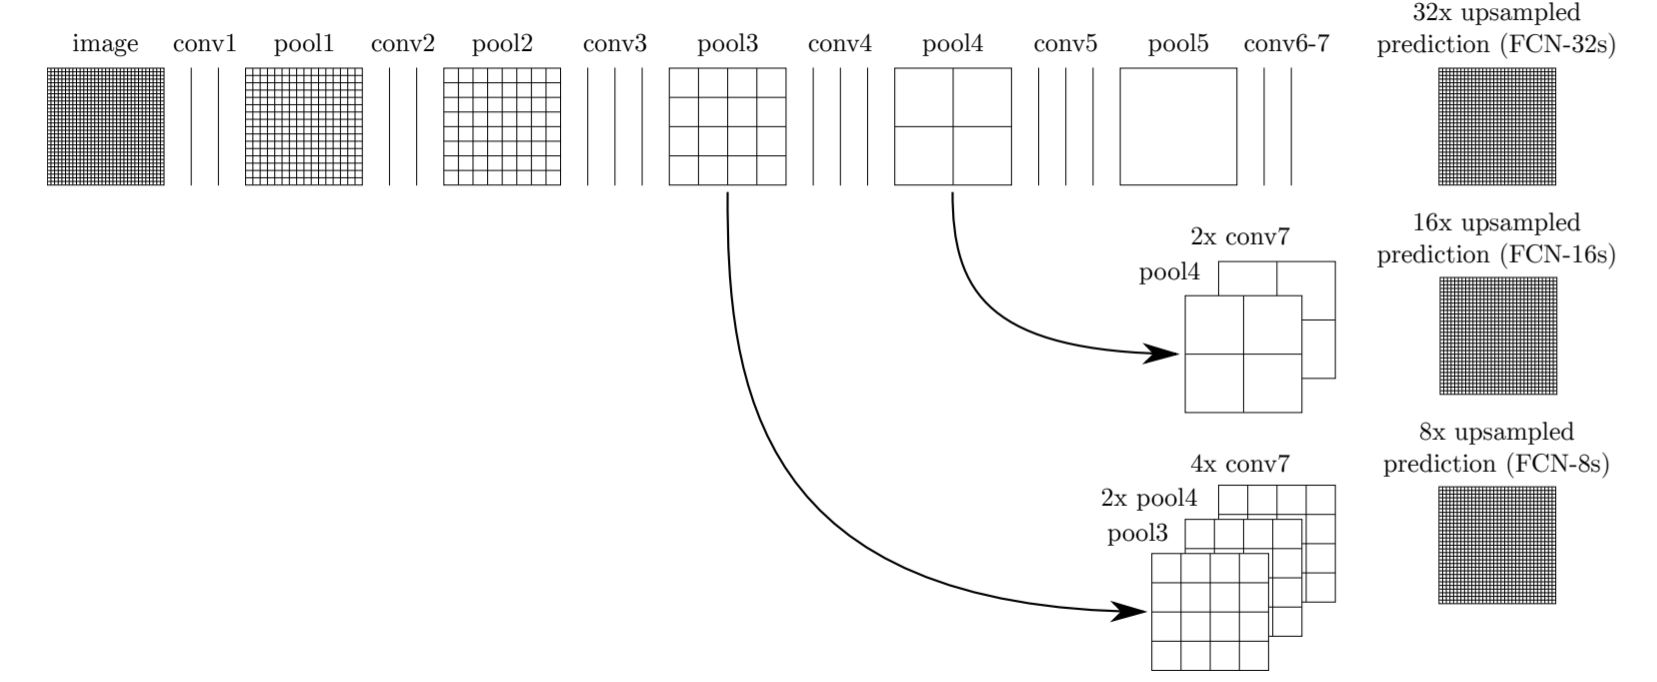
\includegraphics[width=\textwidth]{fcn2.jpg}
\caption{The different variants of the FCN architecture defined in \cite{long2015fully}, with different skip connections added to the base network.}
\end{figure}
\begin{figure}[h]
\centering
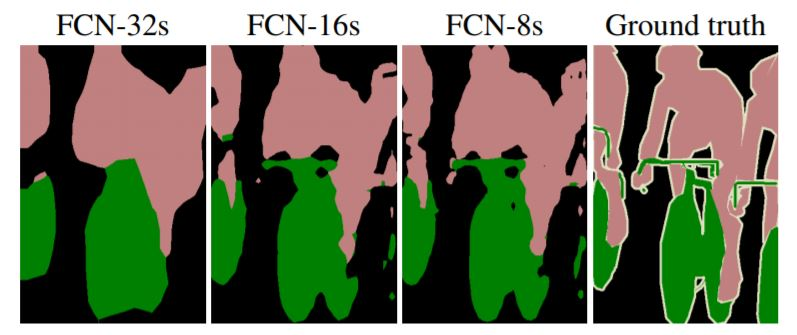
\includegraphics[width=0.6\textwidth]{fcn3.jpg}
\caption{Different networks based on the FCN architecture.}
\cite{long2015fully}
\end{figure}
\newpage

\section{U-Net Architecture}
Proposed by \textit{Ronneberger et al.}\cite{unet}, the U-Net architecture builds upon and extends the FCN architecture for more precise segmentation using a smaller training dataset. While the architecture was designed particularly for bio-medical segmentation applications, it has shown to work well for other domains too.
\begin{figure}[h]
\centering
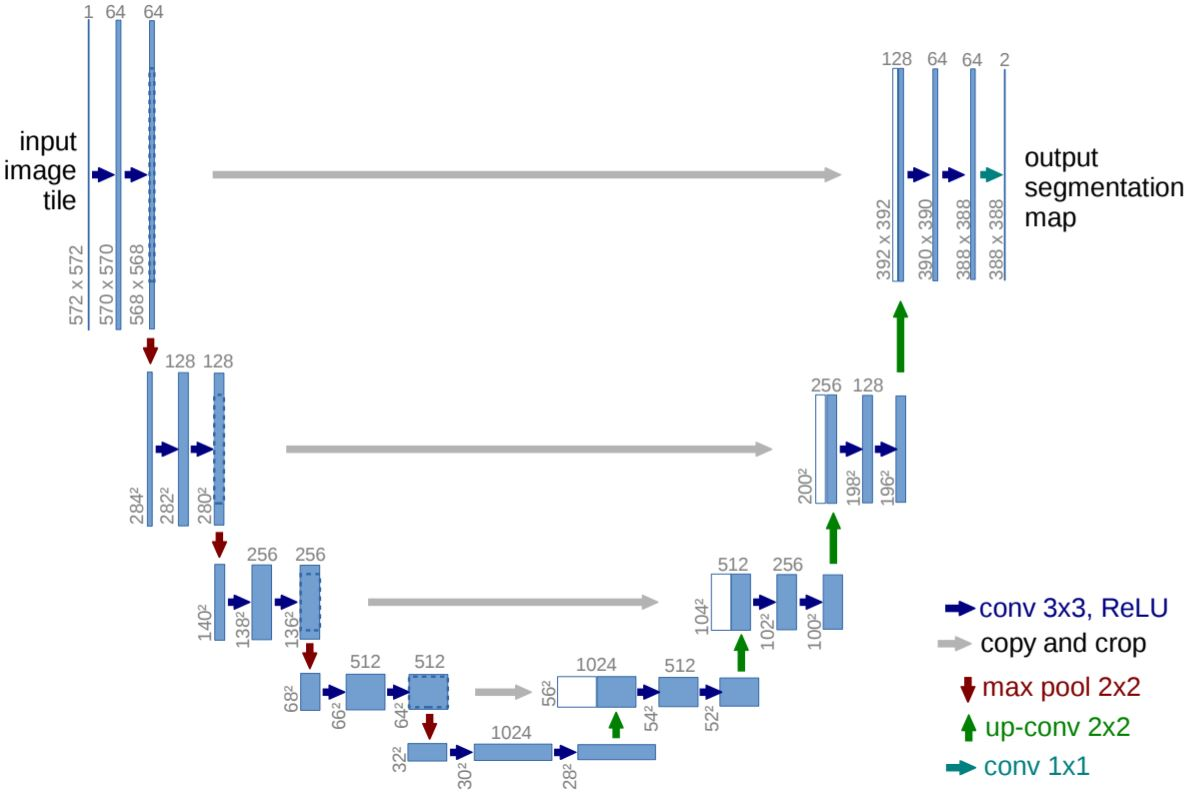
\includegraphics[width=\textwidth]{unet1.jpg}
\caption{The U-Net architecture.}
\cite{unet}
\end{figure}
\subsection{Components}
The U-Net architecture can be divided into three major parts:
\begin{enumerate}
	\item The down-sampling path
	\item The bottleneck
	\item The up-sampling path
\end{enumerate}
\subsubsection{Down-sampling Path}
It is made up of four identical blocks. Each block encloses the following sequence of layers:
\begin{enumerate}
	\item Convolutional layer ($f=3, s=1, p=0$)
	\item Convolutional layer ($f=3, s=1, p=0$)
	\item Max Pooling layer ($f=2, s=2$)
\end{enumerate}
\paragraph{}
At each down-sampling step (max-pooling), the number of channels is doubled, starting with 64 channels in the first block. The down-sampling path captures not only features relevant to classification, but also contextual information about the location of different segments.
\subsubsection{Bottleneck}
It is made up of 2 layers:
\begin{enumerate}
	\item Convolutional layer ($f=3, s=1, p=0$)
	\item Convolutional layer ($f=3, s=1, p=0$)
%dropout
\end{enumerate}
\subsubsection{Up-sampling Path}
It is made up of four identical blocks. Each block encloses the following sequence of layers:
\begin{enumerate}
	\item Up-sampling transpose convolution layer ($f=2, s=2$)
	\item Concatenation with appropriately cropped feature map from down-sampling path
	\item Convolutional layer ($f=3, s=1, p=0$)
	\item Convolutional layer ($f=3, s=1, p=0$)
\end{enumerate}
\paragraph{}
At each up-sampling step (transpose convolution), the number of channels is halved. The output volume after up-sampling is concatenated with the corresponding volume from the down-sampling path after adequate cropping. The introduction of these skip connections allows the propagation of context information about the localization from the down-sampling path to the up-sampling path which already carries semantic information. This helps the network to spread out activations correctly when up-sampling and lends the network its U-shape.
\subsection{Advantages}
The U-Net architecture presented above has several features which lend it better performance than the FCN architecture.
\begin{itemize}
\item
In the FCN architecture, the single up-sampling layer is added at the end of the CNN and has limited number of channels (equal to the number of class labels). The U-Net architecture makes use of multiple up-sampling layers (each with multiple feature channels) in the up-sampling path, interspersed with blocks of convolutional layers. This provides for the opportunity to add more skip connections and so, to fuse contextual and semantic information better, at the time of up-sampling. 
\item
Concatenation is used for combining information from skip connections, as opposed to the summing operation used in the FCN architecture. This helps to retain more information from both sets of activations, without polluting either.
\item
The U-Net architecture is also particularly well suited to applications where labelled training data is not available in abundance. This makes it more attractive for our project on account of the limited computational resources and time available for training the network. We, hence, propose to use this CNN architecture for the problem of land cover classification.
\end{itemize}
\subsection{Disadvantages}
\begin{itemize}
\item Convolutional neural networks do not take temporal variations directly into account. However, it is hoped that providing the network with training data from different time periods should allow it to capture some of the temporal trends.
\item The performance of a deep neural network greatly depends on the amount of training data available. We propose using techniques like data augmentation and transfer learning so as to get better results even with our small training set.
\end{itemize}

% ----------------------------------

% IMPLEMENTATION
\chapter{Implementation}

\section{Data Collection}
\subsection{Google Earth Engine}
Google Earth Engine is a computing platform that allows users to run geo-spatial analysis on Google's cloud infrastructure. It provides several ways to interact with the platform. The Code Editor is a web-based Integrated Development Environment (IDE) for writing and running scripts. The Explorer is a lightweight web app for exploring the data catalog and running simple analyses. The client libraries provide Python and JavaScript wrappers around the web Application Programming Interface (API). The platform provides easy to use tools for handling, visualizing, and extracting large amounts of remote sensing data.\cite{gee1}
\subsection{Datasets}
\subsubsection{Landsat 8}
We are using satellite imagery from the \textit{Landsat 8 - Surface Reflectance - Tier 1} product. The data is collected by Landsat 8 - an American Earth Observation satellite launched in 2013 under Landsat, a joint program of the United States Geological Survey (USGS) and National Aeronautics and Space Administration (NASA). The satellite images the entire Earth's surface at a spatial resolution of 30m, once every two weeks and records multi-spectral and thermal data. The Operational Land Imager (OLI) collects passive remote sensing data from nine spectral bands including the Near Infrared and Visible bands which we intend to use for the project. The data has been atmospherically corrected in addition to standard geometric adjustments and geo-referencing. Information from the thermal infrared sensor is also used to mask clouds. The imagery, hence, provides a clear view of land. The high temporal resolution also helps to factor in temporal variations in land cover. This makes the dataset suitable for the purpose of our project.\cite{geel8, l8}
\subsubsection{Copernicus Global Land Cover dataset}
The \textit{Copernicus Global Land Service (CGLS) - LC100 collection 2} is earmarked as a component of the Land service to operate a multi-purpose service component that provides a series of bio-geophysical products on the status and evolution of land surface at global scale. Derived from the PROBA-V 100m time series data for the year of 2015, this dynamic land cover map at 100 m spatial resolution provides a primary land cover scheme. Next to these discrete classes, the product also includes continuous field layers for all basic land cover classes that provide proportional estimates for vegetation/ground cover for the land cover types.\cite{geecglc}
\subsection{Location}
For training our classifiers, we will be using images of Agra, Mathura and the surrounding region, Uttar Pradesh. This location was chosen as it has a relatively even distribution of different land cover classes. Additionally, first-hand knowledge of the land cover of the region has been provided by the mentor which should help us refine the data. For testing, we will use images of Gandhinagar, Gujarat because of similar reasons.
\begin{figure}[h]
\centering
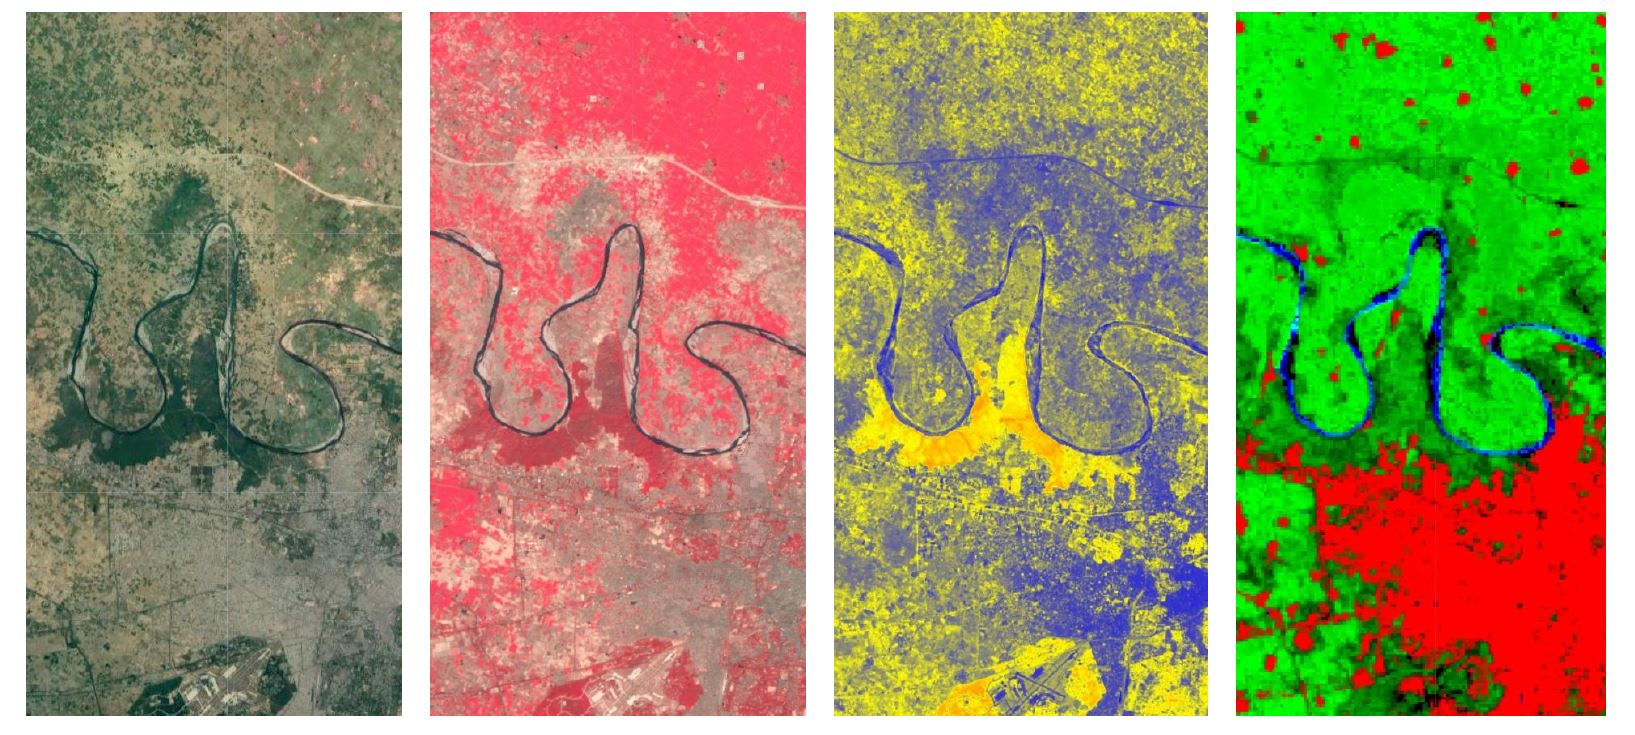
\includegraphics[width=\textwidth]{agra.jpg}
\caption{Different views of the training location - Agra. (1) True colour satellite image (2) False colour infrared image (3) Map of NDVI values (4) Ground truth land cover. [Google Earth Engine]}
\end{figure}

% --------------------------------------

% CONCLUSION
\chapter{Conclusion}

\paragraph{}
Information of land cover classification is very crucial for applications like natural resource management, wildlife habitat protection, urban expansion, damage delineation, target land detection etc. With developments in technology, conventional method of field survey which is both inaccurate and time consuming has been replaced by remotely sensed imagery analysis which is highly accurate and covers wider range. Indian Space Research Organisation (ISRO) and Indian Institute of Remote Sensing (IIRS), Dehradun play an important role in providing information for these applications. Modern statistical and computing techniques like machine learning and deep learning minimize the human intervention in the task of analysis and classification, thus making the outcome very accurate and the process very agile.
\paragraph{}
The project seeks to compare the applicability of machine learning and deep learning techniques to the problem of land cover classification. Support Vector Machines are traditional machine learning models that provide a method for pixel-wise classification based on learning from the temporal variations in the NDVI time series. On the other hand, Convolutional Neural Networks - a class of deep neural networks, use the spatial variations in the infrared and visible bands of the satellite image for segmentation. The two, hence represent very different approaches for solving the problem. However, the project is still at a very nascent stage, and any comment regarding the comparative performance of these two approaches cannot be made yet.

% ---------------------------------------

% REFERENCES
\printbibliography[heading=bibintoc, title={References}]

\section{Glossary}
Chlorophyll- Green photosynthetic pigment found in plants\\
CNN- Convolutional Neural Networks\\
Convolution- mathematical way of combining two signals to form a third signal\\
ET- Evapotranspiration\\
FCN- Fully Convolutional Neural Network\\
GEE- Google Earth Engine\\
GPU- Graphical Processing Unit\\
IIRS- Indian Intitute of Remote Sensing\\
kernel- Kernel functions.\\
Landsat 8- an American Earth observation satellite launched on February 11, 2013.\\
NDVI- Normalised Difference Vegetation Index\\
NIR- Near-Infrared\\
NN- Neural Networks.\\
Pixel- a minute area of illumination on a display screen, one of many from which an image is composed.\\
Pooling- process of extracting features from image output of a convolution layer\\
Semantic Segmentation-the process of associating each pixel of an image with a class label\\
SVM- Support Vector Machines\\
Temporal- relating to time\\





\end{document}
